\startchapter{Possibilities for Treating Experimental Data} \label{ch:6}
\section{Description}
The experimental spectra obtained from Raman or SFG techniques are often measured in arbitrary intensity units, which results an amplitude scaling factor when compared to the candidate spectra generated mathematically. In other words, this means that between candidates' theoretical spectra and the experimental one, there is an unknown scaling factor, same applied to IR. Within one particular spectroscopy technique, the scaling factor is the same for all the polarizations. Take IR absorption as an example. The scaling factor for the spectrum of $x$-polarization is the same as the one for the spectrum of $z$-polarization. Therefore, it is necessary to consider this scaling factor when using the spectral information to build the LP instances. \\

\section{Test Case}
The first part of this section, we study the cases where each molecule's candidates expanded in $[0^{\circ}$, $90^{\circ})$ on $\theta$ to see which spectral information is sufficient in obtaining the target composition when scaling factor is considered. Then in the second part, we study the cases where each molecule's candidates expanded from $[0^{\circ}$, $180^{\circ}]$ on $\theta$, excluding $90^{\circ}$. \\

\subsection{Test Cases with Scaling Factor Considering Each Amino Acid Candidates Expanded in $[0^{\circ}$, $90^{\circ})$ on $\theta$ in a Mixture of Amino Acids}
In Chapter \ref{ch:5}, as long as the constructed instances of our LP model contain Raman or SFG spectral information, the LP solver returns the target composition when candidates for each amino acid expanded in $[0^{\circ}$, $90^{\circ})$ on $\theta$ in a mixture of amino acids. Therefore, based on these test cases, we investigate whether the LP instances built by using the experimental data return the target composition.\\

Therefore, the same test cases in Table \ref{tab:5.1} are used. The goal is the same, figuring out which spectral information is sufficient to retrieve the target composition for the mixture of six amino acids' candidates. The only difference is that, in each run of the test cases, an arbitrary scaling factor is generated for IR, Raman and SFG, respectively. Therefore, the target spectra are not only composed by the target composition of all candidates, but also need to multiple by the randomly generated scaling factors of each spectroscopy technique. \\

To start with, we limit the scaling factors to be smaller than 1. After a few runs of the test cases, it is observed that the returned compositions always contains one extra variable in every test case. For Cases 2, 4, 6 and 7, the returned composition contains the correct selected candidates. However, the percentage values of the selected candidates are different from the target composition. The ratio between the returned percentage and the target percentage is the same for all the selected candidates. Furthermore, we add this ratio to the extra variable which equals $1$. We randomly select one run of the test cases as an example. Figure \ref{fig:6.2} displays the target composition, only the selected candidates are annotated with assigned percentage. Figure \ref{fig:6.2} displays the return composition of Case 2. The selected candidates in the return composition are correct. However, each percentage value is different from the one in the target composition. There is one extra value in Figure \ref{fig:6.2} with a value of $0.4$. \\

\begin{figure}[!ht] 
\centering
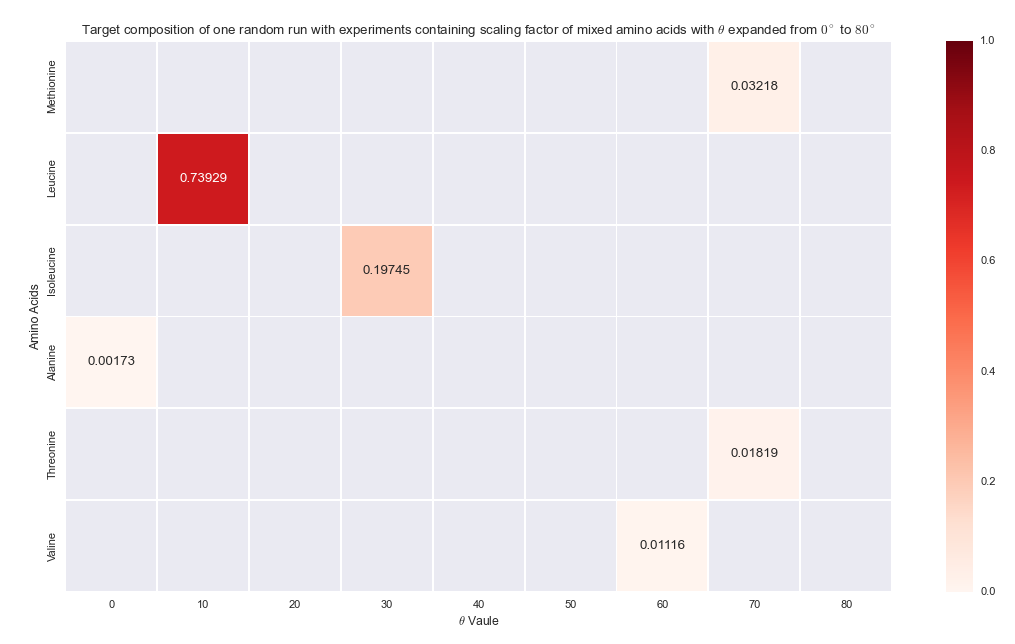
\includegraphics[scale=0.7]{Figures/chapter6_figure_one.png}
\caption{Target composition for one random run of the test case set with scaling factor for mixed amino acids, with $\theta$ expanded in $[0^{\circ}$, $90^{\circ})$. More detailed data of this target composition can be found in Appendix \ref{eqn:A.4}.} \label{fig:6.1}
\end{figure}

\begin{figure}[!ht] 
\centering
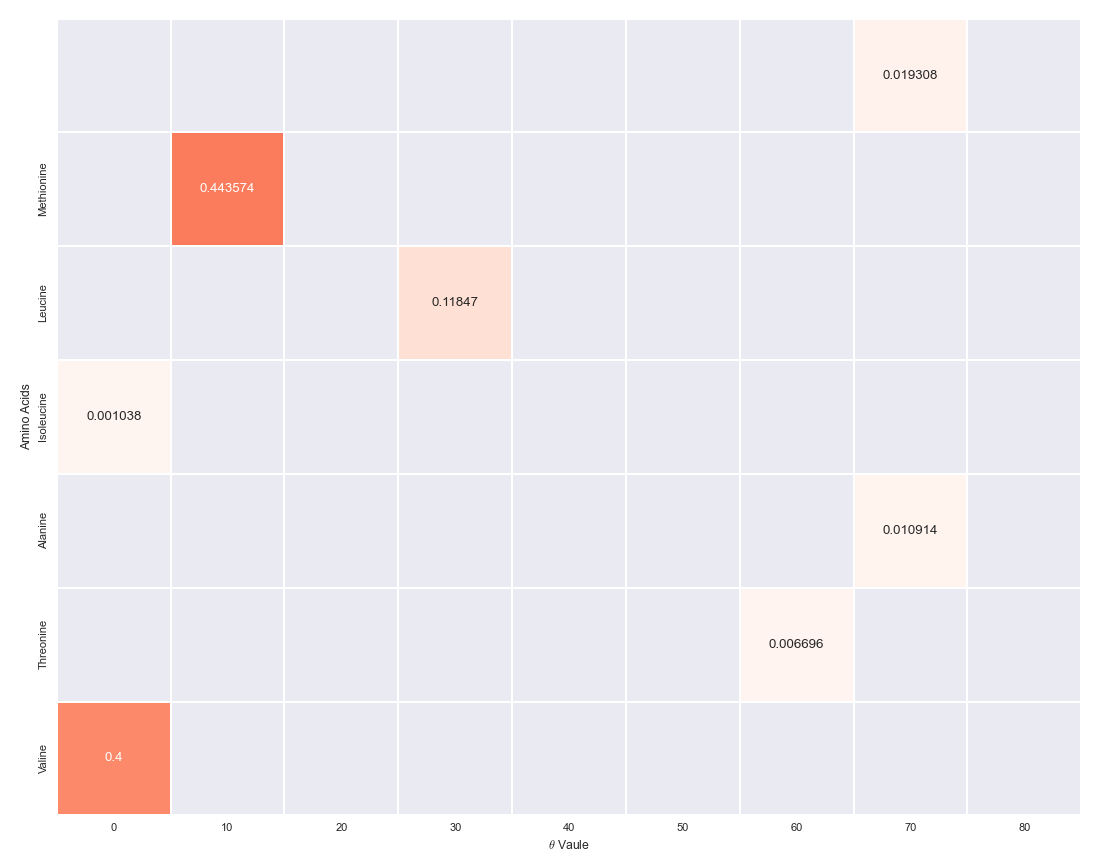
\includegraphics[scale=0.7]{Figures/chapter6_figure_two.png}
\caption{Return composition of Case 2 for one random run of the test case set with scaling foctor for mixed amino acids, with $\theta$ expanded in $[0^{\circ}$, $90^{\circ})$. More detailed data of this target composition can be found in Appendix \ref{eqn:A.5}.} \label{fig:6.2}
\end{figure}

%\begin{figure}[!ht] 
%\centering
%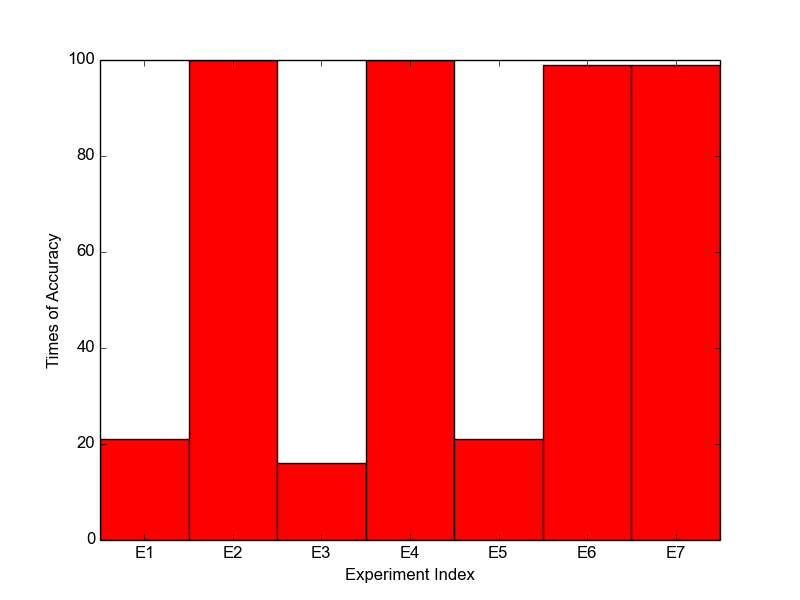
\includegraphics[scale=0.6]{Figures/chapter6_1.png}
%\caption{Test case accuracy analysis for test cases using experimental spectra data that contains scaling factor that is smaller than 1 and candidates with $\theta$ expanded in  $[0^{\circ}$, $90^{\circ})$.}
%\label{fig:6.3}
%\end{figure}

Moreover, Equation \ref{eqn:6.3} shows the ratio between the percentages of the selected candidates in the return composition and the target one is the same for all the amino acids (more detailed calculated can be found in Appendix \ref{eqn:A.9}). The value of this ratio is $0.6$. When this ratio is added up with the extra variable (referred to as slack variable (SV) in LP) $0.4$, the total is $1$. The scaling factors are randomly generated in our test cases. In this run of test cases, the scaling factor for Raman spectra is $0.6$. In conclusion, the SV is returned by LP. Then the scaling factor (SF) equals to $1 - SV$. From the scaling factor, the ratio between the return composition and the target one is known. At the end, the target composition can be re-built from the ratio and the return composition. The re-constructed target composition matches the original one. \\

\begin{eqnarray} \label{eqn:6.3}
\frac{0.019}{0.032} = \frac{0.44}{0.74} = \frac{0.12}{0.2} =\frac{0.001}{0.0017}  = \frac{0.011}{0.018} = \frac{0.0067}{0.011} = 0.6
\end{eqnarray}

To verify if the above observation can be generalized, the test cases in Table \ref{tab:5.1} are run 100 times with randomly generated scaling factors in each run. Table \ref{tab:6.1} indicates the result of these test cases. Cases 2, 4, 6 and 7 meet the above observation with almost $100\%$ frequency. This indicates that even with the scaling factor, Raman spectral information alone is sufficient to study the mixed molecules' orientation distribution at surfaces when each amino acid's candidates expanded in $[0^{\circ}$, $90^{\circ})$ on $\theta$. The target composition can be re-constructed correctly from the return slack variable and the return composition. Table \ref{tab:6.1} also illustrates that Case 3 does not hit the above observation with high frequency. With the scaling factor as the addition, SFG spectral information alone is not sufficient to obtain the target composition. Case 5 indicates that even combining IR and SFG spectral information, the constructed LP model cannot help to reconstruct the target composition. This can be caused by the different scaling factors of these two spectroscopy techniques. \\

\begin{table}[ht!]
\begin{center}
{\def\arraystretch{1.5}
\begin{tabular}{| l | l | l | l | l | l | l | l |}
\hline
Test Case & 1 & 2 & 3 & 4 & 5 & 6 & 7 \\ \hline
\# of Returning Target Composition& 2 & 100 & 17 & 100 & 21 & 98 & 98 \\ \hline
\end{tabular} 
}
\end{center}
\caption{The number of each test case returns the target composition when experimental spectra data is used, and the candidates of each amino acid expanded in $[0^{\circ}$, $90^{\circ})$ on $\theta$.}
\label{tab:6.1}
\end{table}	


\subsection{Test Cases with Scaling Factor Considering Each Amino Acid Candidates Expanded in $[0^{\circ}$, $180^{\circ}]$ on $\theta$ in a Mixture of Amino Acids}
When each amino acid's candidates are expanded in $[0^{\circ}$, $180^{\circ}]$ on $\theta$, excluding $90^{\circ}$, the same set of test cases is run 100 times with randomly generated scaling factors in each run. The result of each test case in $100$ run shows that all test cases hit the previous observation with zero frequency. \\

However, when we further analyze the return compositions of Cases 2 and 6, there are few other observations to be noted. To facilitate the explanation, one random run is picked as an explicit example. Figure \ref{fig:6.4} is the target composition. Figure \ref{fig:6.5} and Figure \ref{fig:6.6} are the return compositions of Case 2 and Case 6. The generated scaling factor for IR, Raman and SFG are $0.86$, $0.77$ and $0.24$. \\

In Figure \ref{fig:6.5}, in the return composition of Case 2, the slack variable equals $1-SF = 1-0.77 = 0.23$. For each amino acid, the selected candidate in the return composition may not be the exact one as shown in the target composition. However, this selected candidate is always either the one with correct $\theta$, or $180^{\circ}-\theta$. Moreover, the ratio between the percentage of each selected candidate in Figure \ref{fig:6.5} and Figure \ref{fig:6.4} are the same as shown in Equation \ref{eqn:6.2} (more detailed calculated can be found in Appendix \ref{eqn:A.10}). These ratios all equal to the scaling factor of Raman. \\

In Figure \ref{fig:6.5}, for each amino acid, there are two selected candidates in the return composition. These two selected candidates are the one of correct $\theta$ and $180^{\circ}-\theta$. When the percentages of these two selected candidates are added, it equals to the percentage returned for the amino acid in Figure \ref{fig:6.4}, $0.27 + 0.14 = 0.41$. Between these two selected candidates, the correct one's percentage is always larger' than its $\theta$ complement, $0.27 > 0.14$. In conclusion, we observe Case 2 returns the slack variable, the scaling factor, and we can obtain the ratio between the returned candidates and the target ones. However, in order to distinguish the exact candidate of each amino acid, the extra information from Case 6 is required. Case 6 tells the correct candidate from the one with $\theta$ complement. Together with the return information from Case 2 and 6, the target composition can be obtained. In another way, only analysing the return composition of Case 6 also helps us to deduce the target composition as well. These observations can be applied to every run of the set test cases.\\


\begin{figure}[!ht] 
\centering
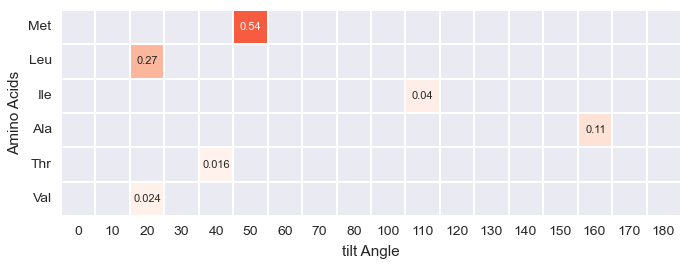
\includegraphics[scale=0.7]{Figures/chapter6_figure_five.png}
\caption{Target composition of one random run of test cases containing scaling factor and the mixed amino acids' candidates with $\theta$ expended in $[0^{\circ}$, $180^{\circ}]$. More detailed data of this target composition can be found in Appendix \ref{eqn:A.6}.} \label{fig:6.4}
\end{figure}

\begin{figure}[!ht] 
\centering
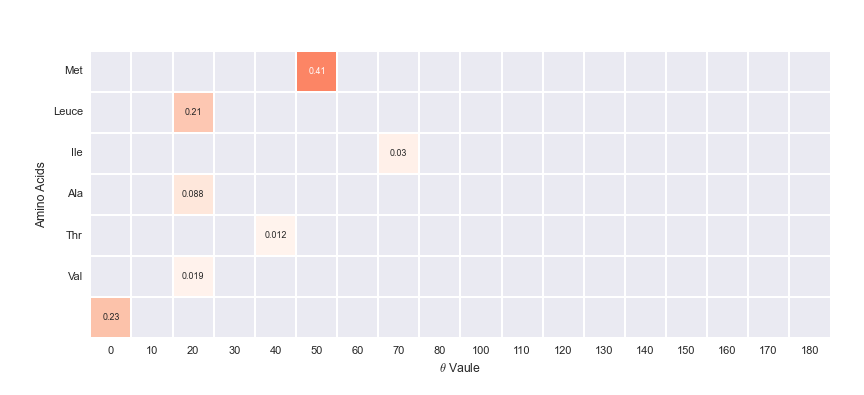
\includegraphics[scale=0.7]{Figures/chapter6_figure_three.png}
\caption{Return composition of Case 2 for one random run of test cases containing scaling factor and the mixed amino acids' candidates with $\theta$ expended fin $[0^{\circ}$, $180^{\circ}]$. More detailed data of this target composition can be found in Appendix \ref{eqn:A.7}.} \label{fig:6.5}
\end{figure}

\begin{figure}[!ht] 
\centering
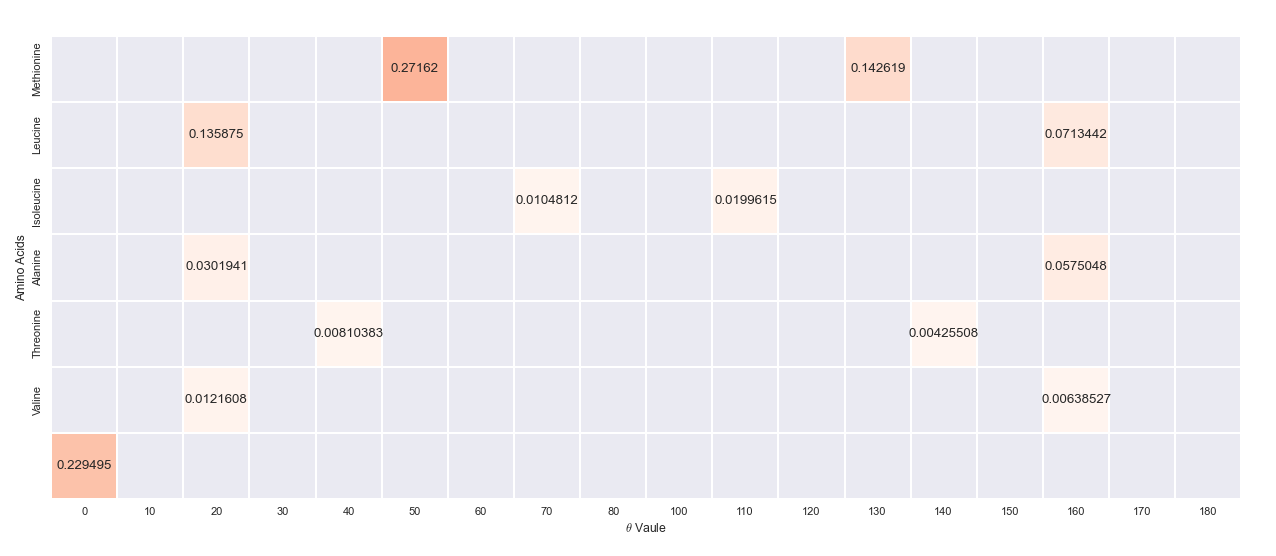
\includegraphics[scale=0.7]{Figures/chapter6_figure_four.png}
\caption{Return composition of Case 6 for one random run of test cases containing scaling factor and the mixed amino acids' candidates with $\theta$ expended in $[0^{\circ}$, $180^{\circ}]$. More detailed data of this target composition can be found in Appendix \ref{eqn:A.8}.} \label{fig:6.6}
\end{figure}

\begin{eqnarray} 
\begin{split}
\frac{0.41}{0.54} &= \frac{0.21}{0.27} = \frac{0.03}{0.04}  =\frac{0.088}{0.11} = \frac{0.012}{0.016} = \frac{0.019}{0.024} = 0.77
\end{split}\label{eqn:6.2}
\end{eqnarray}

\section{Conclusion}

With the introduction of the scaling factor to different spectroscopy techniques, Raman spectral information alone is sufficient to obtain the target composition, when considering a mixture of amino acids with candidates expanded in $[0^{\circ}$, $90^{\circ})$ on $\theta$. The target composition can be re-constructed from the return SV and composition. The SF equals 1 minus SV. \\

When each amino acid's candidates are expanded in $[0^{\circ}$, $180^{\circ}]$, both return compositions of using only Raman and SFG spectral information is needed to obtain the target composition.  \\
